\textbf{(DRAFT)} Crystallography question on a YBCO\footnote{Speaking of which, my friend has recently recommended me this awesome video of someone growing a YBCO superconductor \textit{by himself}: \url{https://www.youtube.com/watch?v=sLFaa6RPJIU}} crystal.
\begin{parts}
	\part If all oxygen sites are fully occupied, we have an occupancy of $8$.
	
	However for $\delta = 0.5$, the occupancy would be $6+0.5 = 6.5$.
	
	\begin{figure}[H]
		\centering
		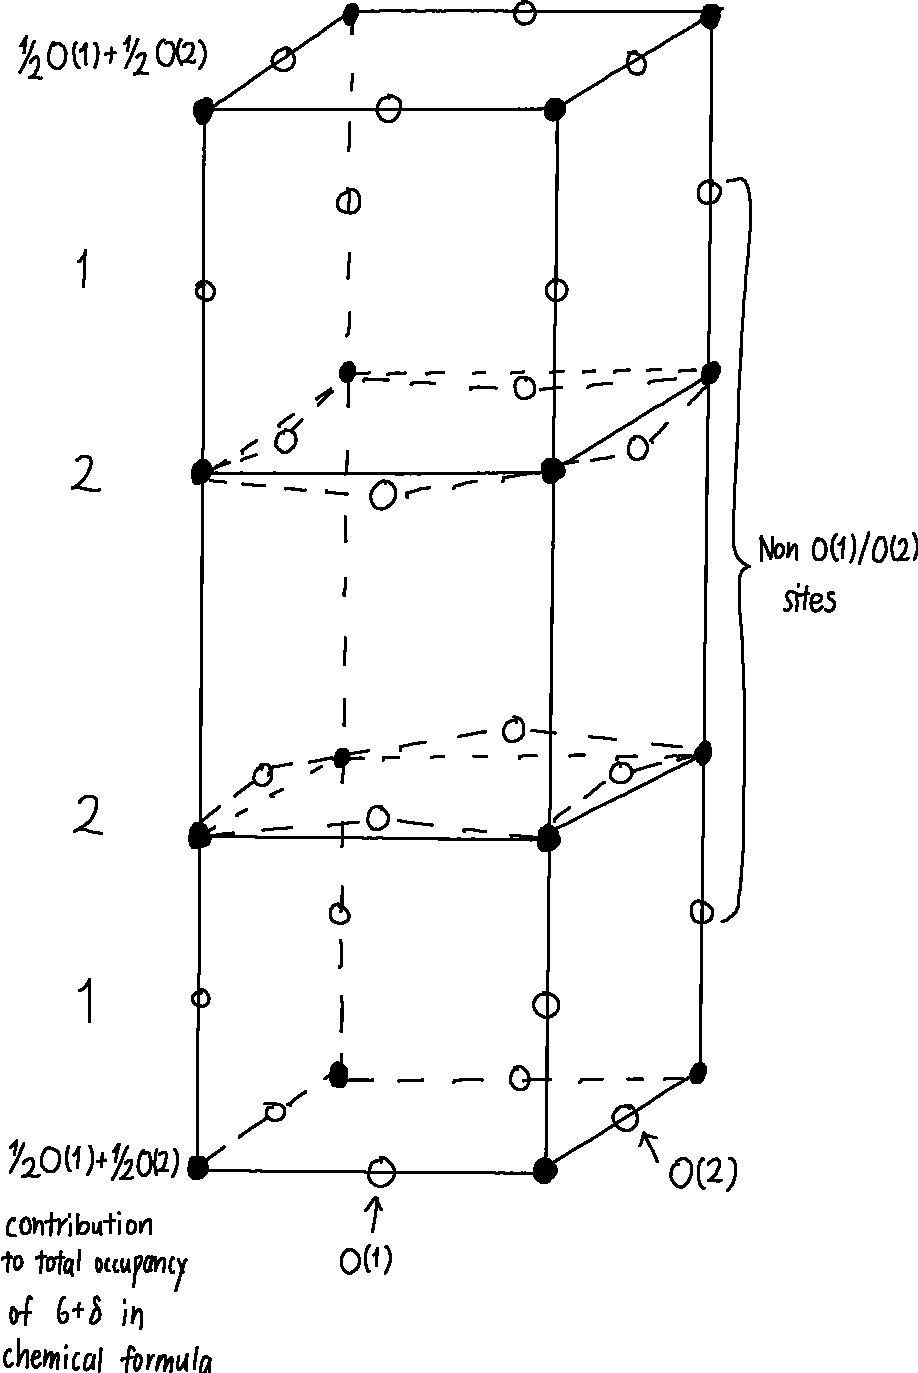
\includegraphics[width=.75\linewidth]{q1-occupancy}
	\end{figure}
	
	With the sketch as aid (ignoring Y and Ba atoms), we proceed to find the average fractional occupancy $f$ of the degenerate O(1)/O(2) sites:
	\begin{gather*}
		2f = 0.5 \\
		\Rightarrow f = 0.25
	\end{gather*}
	
	\part Drawing out tetragonal symmetry elements should do the job.
	\begin{subparts}
		\subpart \textbf{(TO BE VERIFIED)}
		Naturally we have a 4-fold axis about the c-axis about $\left(\frac{1}{2},\, \frac{1}{2}\right)$.
		
		\begin{figure}[H]
			\centering
			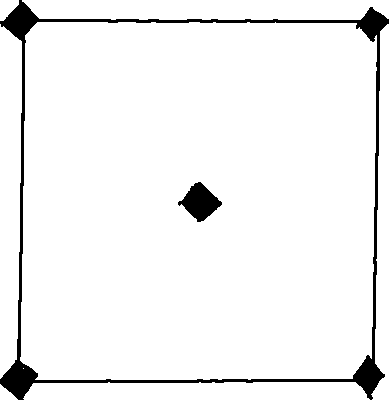
\includegraphics[width=.25\linewidth]{q1-symmetry-rotation}
		\end{figure}
		
		\subpart Mirror planes along a/b axes and the diagonals, and a $m_z$ at $c=\diagfrac{1}{2}$.
		\begin{figure}[H]
			\centering
			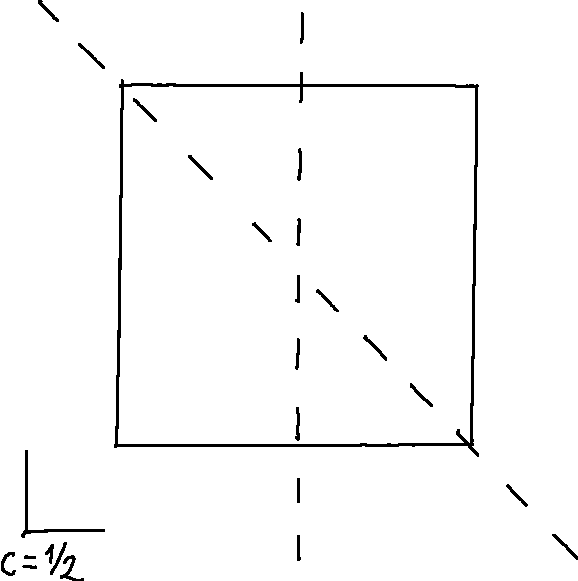
\includegraphics[width=.4\linewidth]{q1-symmetry-mirror}
		\end{figure}
		
		\newpage
		\subpart Glide plane of $m_x$ with translation of $\diagfrac{1}{2}$ along the c-axis.
		\begin{figure}[H]
			\centering
			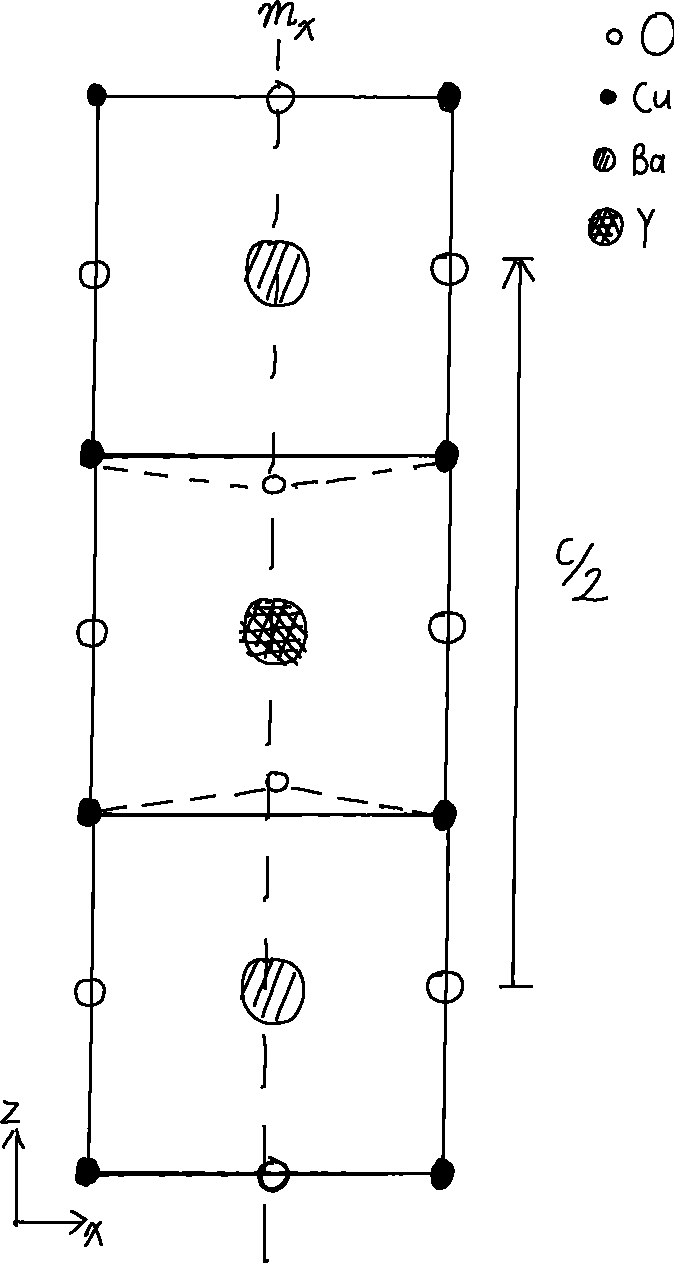
\includegraphics[width=.5\linewidth]{q1-symmetry-glide}
		\end{figure}
	\end{subparts}
	
	\part As the crystal undergoes transition from tetragonal to orthorhombic structure, the symmetry between a and b axes is lost.
	
	Therefore of all the symmetry elements listed in part b, the 4-fold rotation axes and the diagonal mirror plane are no longer present.
	
	\newpage
	\part Sketches of $z=0$ layer illustrating the domains:
	\begin{figure}[H]
		\centering
		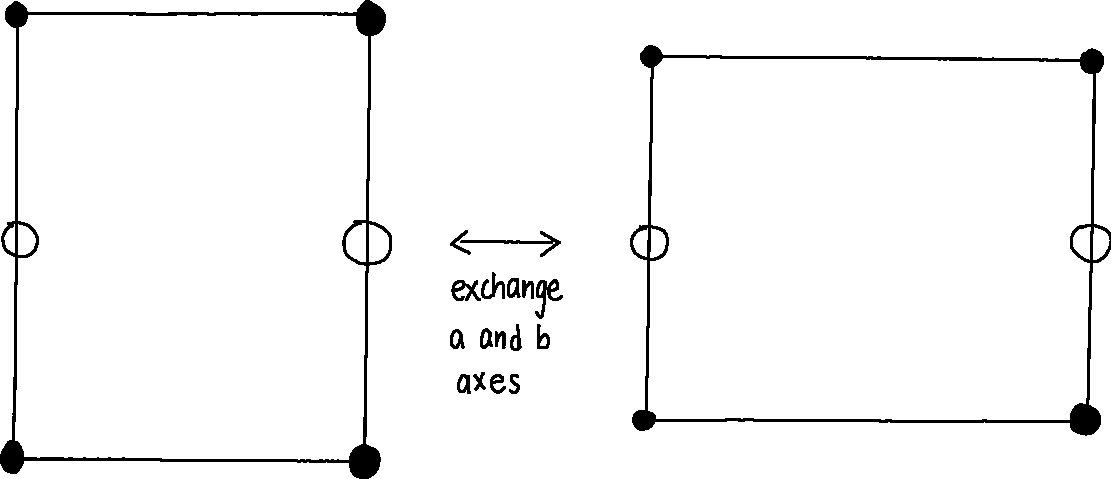
\includegraphics[width=.5\linewidth]{q1-domains}
	\end{figure}
	
	Sketches illustrating twinning structures:
	\begin{figure}[H]
		\centering
		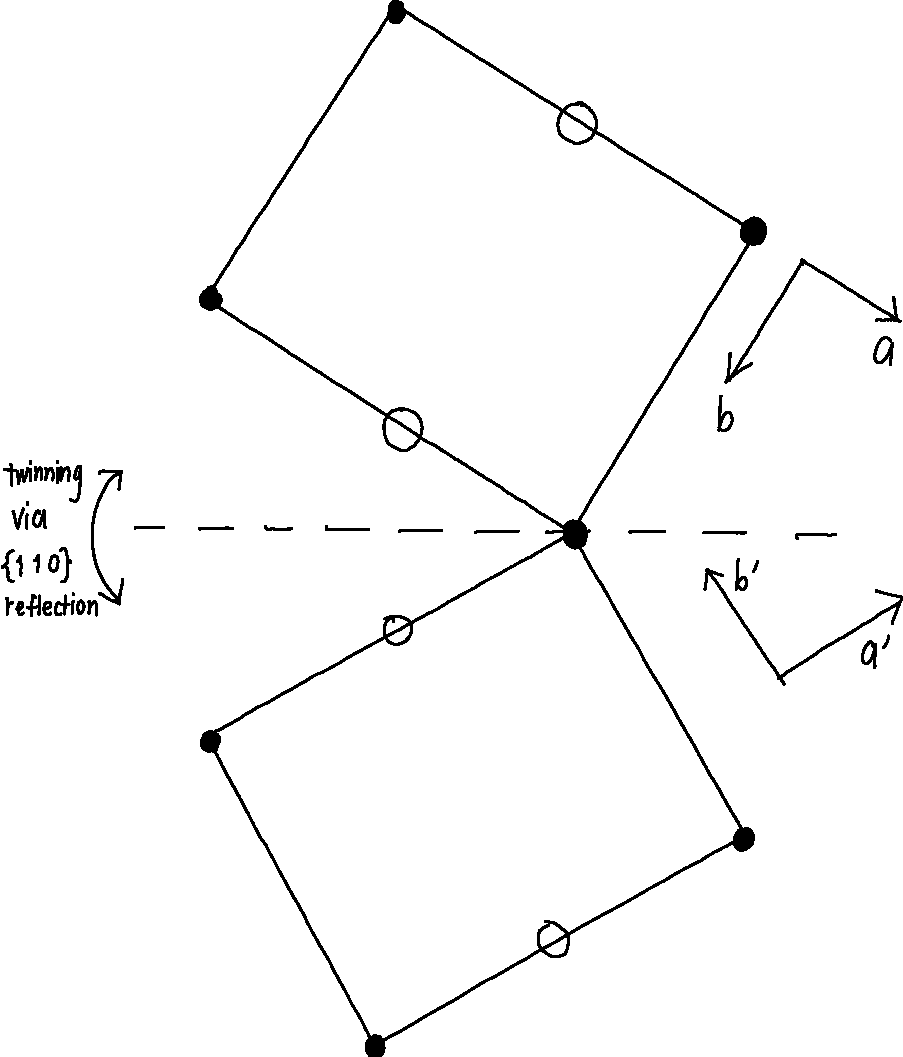
\includegraphics[width=.4\linewidth]{q1-twinning-1}
		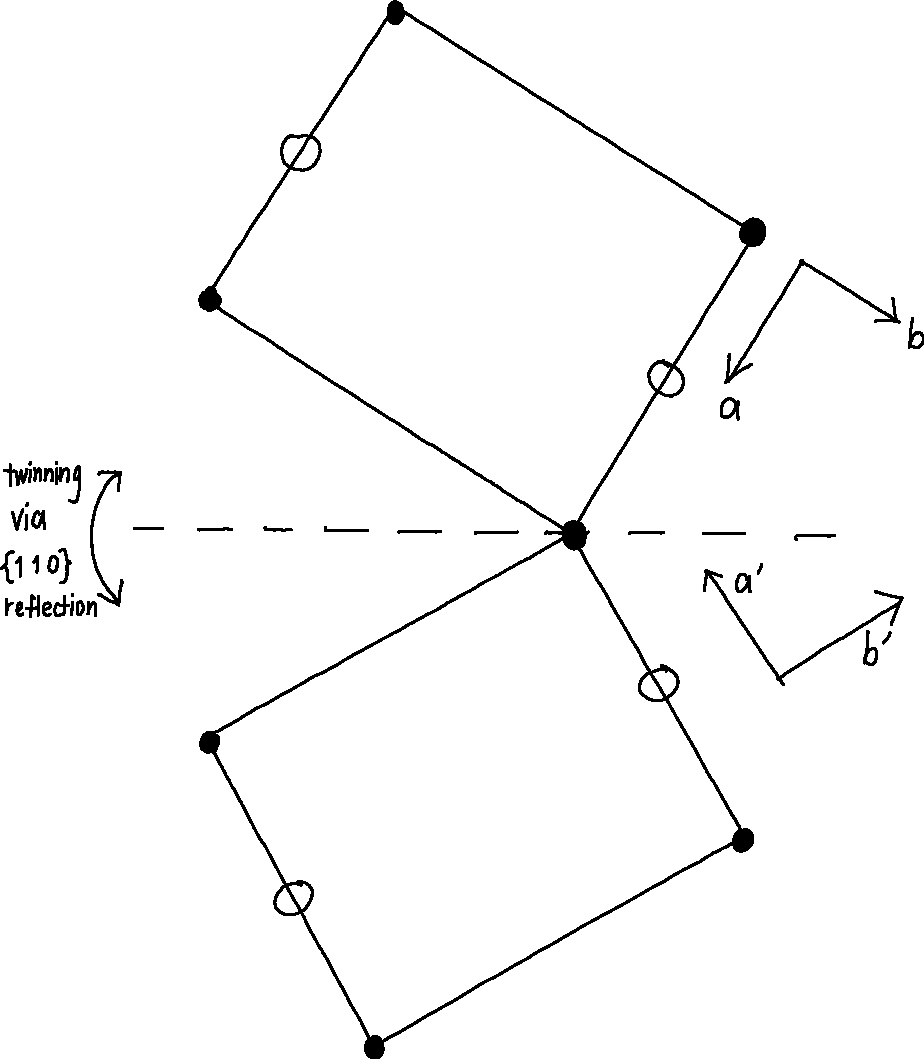
\includegraphics[width=.4\linewidth]{q1-twinning-2}
	\end{figure}
	
	\part \textbf{(TO BE VERIFIED)}
	As mentioned above, when the YBCO undergoes transition from the tetrahedral to the orthorhombic structure, it loses the symmetry between the $a$ and $b$ axes.
	This gives rise to the splitting of the $(h00)$ and the $(0k0)$ peaks.
	
	In addition, a crystal may also possess structural defects such as domains and micro-twins as described above.
	This introduces the asymmetry in the crystal, thereby causing further splits in the peaks -- there should be $3$ split peaks for each orthorhombic sub-peak from the reflection in the $(110)$ and $(\bar{1}10)$ planes.
	
	In total we then may have up to $6$ split peaks.
\end{parts}